\subsection{実務上の考慮}

構築は、現実の制約の中で進む。要求は変わり、設計は不完全で、利用できる人員や時間には限りがあり、外部サービスやライブラリにも制約がある。そのため、構築は理論だけでなく、実務的な判断が重要な活動である。

\subsubsection{構築設計}

構築段階でも設計は行われる。要求分析や上位設計で決まっていない詳細を、構築中に決める必要があるためである。たとえば、アルゴリズム、データ構造、関数やクラスの責務、インタフェース、例外の扱い、ログの粒度などは、構築中に具体化されることが多い。

建築現場で、図面に書かれていない細部を現場で調整する必要があるのと同じで、ソフトウェア構築でも詳細の調整が必要である。ただし、場当たり的に決めるのではなく、設計原則、標準、テスト容易性、変更容易性に基づいて判断する必要がある。

\subsubsection{構築言語}

構築言語とは、人間がコンピュータに実行可能な解決策を指定するための言語である。狭い意味のプログラミング言語だけでなく、設定言語、ツールキット言語、スクリプト言語、ドメイン固有言語も含む。

\par\smallskip\noindent\refstepcounter{table}\label{tab:ch04-03}表 \thetable: 構築言語の整理\par\smallskip
表 \thetable は、構築言語の整理を比較・確認しやすい形で整理したものである。\par\smallskip
\begin{longtable}{L{0.24\linewidth}L{0.66\linewidth}}
\toprule
構築言語の種類 & 説明 \\
\midrule
設定言語 & 限られた選択肢から設定を選び、ソフトウェアの振る舞いや導入形態を変える言語である。設定ファイルなどが該当する。 \\
ツールキット言語 & 特定の部品群やツールキットを組み合わせてアプリケーションを作るための言語である。 \\
スクリプト言語 & 自動化、処理の連結、簡易アプリケーションの構築によく使われる言語である。 \\
プログラミング言語 & 汎用的で柔軟な構築言語である。C/C++、Java、Python、C\# などが例である。 \\
ドメイン固有言語 & 特定の業務領域や技術領域の概念を直接表す言語である。汎用言語よりも領域内の問題を簡潔に表せることがある。 \\
\bottomrule
\end{longtable}

構築言語の表記法には、テキストを中心にする言語的表記、数学的に厳密な形式的表記、図形やアイコンを中心にする視覚的表記がある。言語選択は、性能、信頼性、移植性、セキュリティ、開発者の学習コストに影響する。

\par\smallskip
\begin{center}
\centering
\IfFileExists{assets/generated_figures/ch04/fig-ch04-06.png}{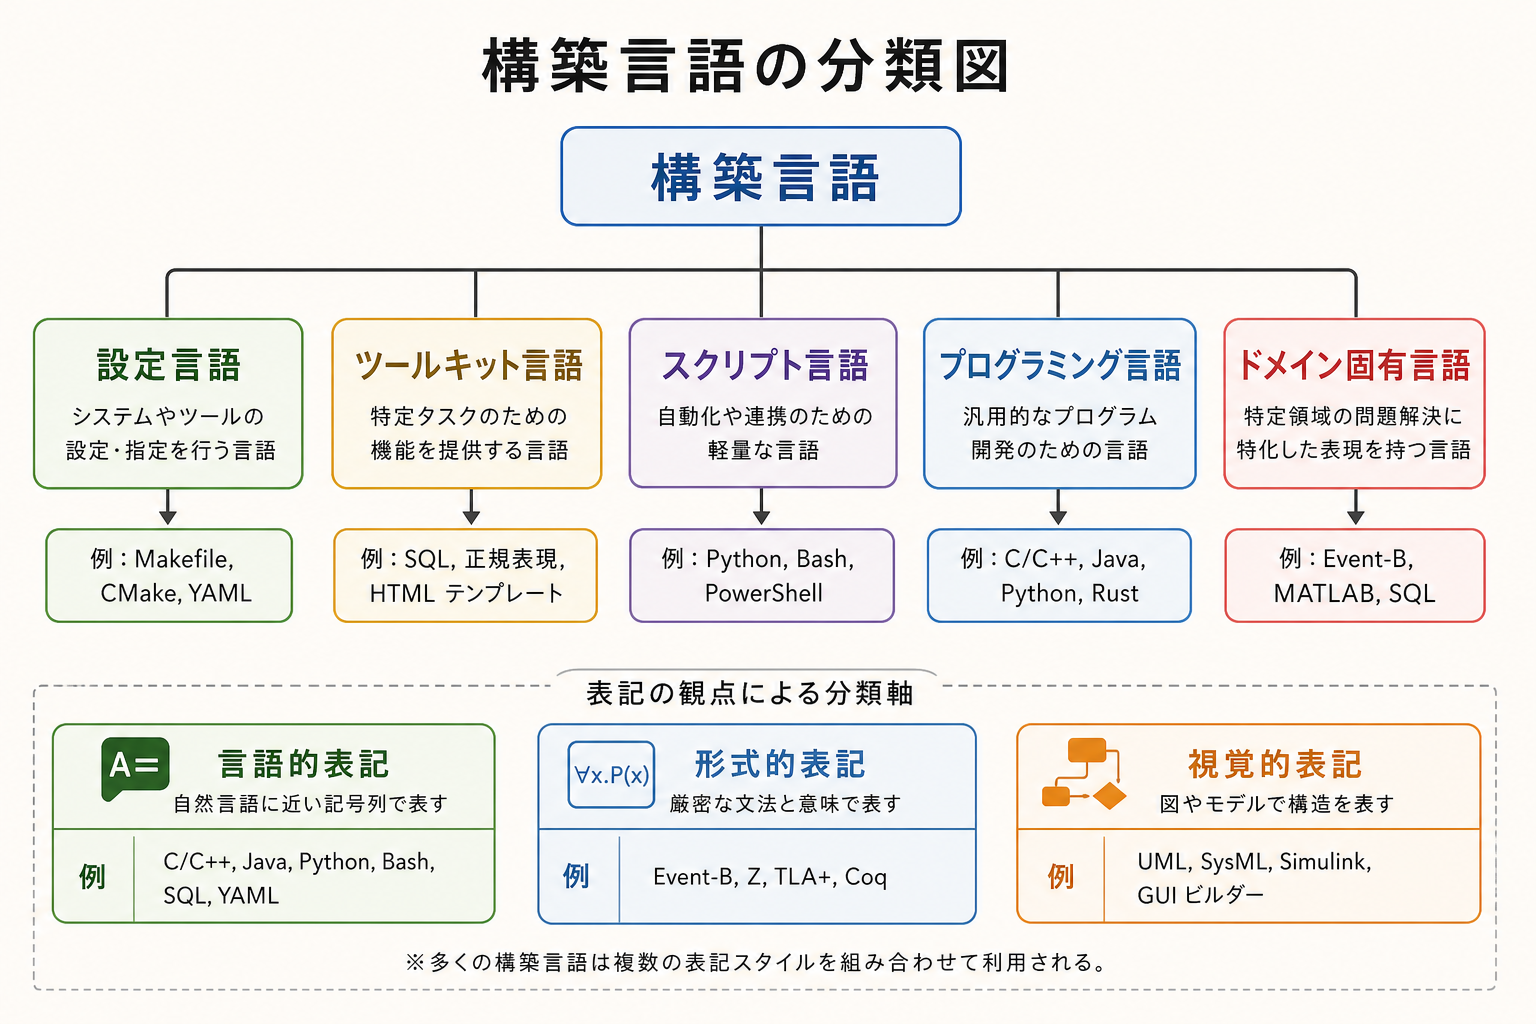
\includegraphics[width=0.96\linewidth]{assets/generated_figures/ch04/fig-ch04-06.png}}{\fbox{\parbox[c][48mm][c]{0.9\linewidth}{\centering 画像生成待ち\\構築言語の分類図}}}
\par\smallskip
\refstepcounter{figure}\label{fig:ch04-06}図 \thefigure: 構築言語の分類図
\end{center}
図 \thefigure は、構築言語の分類図を視覚的に整理したものである。
\par\smallskip

\subsubsection{コーディング}

コーディングでは、ソースコードを理解しやすく、変更しやすく、検証しやすく書くことが重要である。単に動作するコードを書くだけでは不十分である。コードは、将来の読者に意図を伝える文書でもある。

構築におけるコーディングの主な考慮事項は次のとおりである。

\begin{itemize}
  \item 命名規則、字下げ、レイアウトにより、理解しやすいソースコードを作る。
  \item クラス、列挙型、変数、名前付き定数などを適切に使う。
  \item 条件分岐、ループ、例外処理などの制御構造を過度に複雑にしない。
  \item 予期できるエラーと例外的なエラーを区別して扱う。
  \item バッファオーバーフロー、配列範囲外参照、入力検証不足など、コードレベルのセキュリティ問題を防ぐ。
  \item スレッド、データベースロック、ファイル、ネットワーク接続などの資源を適切に扱う。
  \item コードを関数、クラス、パッケージなどに整理する。
  \item 必要な文書化とコメントを行う。
  \item 測定に基づいて性能を調整する。
\end{itemize}

\begin{keybox}{コメントの考え方}
コメントは、コードの日本語訳ではない。よいコメントは、コードだけでは読み取りにくい理由、前提、制約、例外、意図を説明する。名前と構造で伝えられることは、名前と構造で伝える方がよい。
\end{keybox}

\subsubsection{構築テスト}

構築では、主に単体テストと統合テストが行われる。これらは、多くの場合、コードを書いたソフトウェア技術者自身が実行する。構築テストの目的は、欠陥が混入してから発見されるまでの時間差を短くし、修正費用を下げることである。

単体テストは、関数、クラス、モジュールなどを単独で確認する。統合テストは、それらを組み合わせたときに正しく相互作用するかを確認する。構築テストは、通常、システムテスト、アルファテスト、ベータテスト、ストレステスト、使用性テストなどの広い範囲のテストまでは含まない。

\term{テストケース}{Test Case}は、コードを書いた後に作られることもあるが、コードを書く前に作られることもある。テストを先に書く方法は、テストファーストプログラミングまたはテスト駆動開発として扱われる。

\subsubsection{構築における再利用}

構築における再利用には、再利用のための構築と、再利用による構築がある。再利用のための構築では、将来別の場所で使えるように、部品を作る。可変性を設定で変えられるようにする、使い方を文書化する、単体テストを整備する、公開方法を整えるといった作業が必要である。

再利用による構築では、既存の部品を使って新しいソフトウェアを作る。ライブラリ、フレームワーク、オープンソース部品、商用既製品、クラウドサービスが代表例である。クラウドサービスを利用する場合、認証、メッセージング、ストレージなどを外部のサービスへ委任できる。このような形は、バックエンドサービスとしての利用とも呼ばれる。

再利用では、部品を選び、評価し、統合し、テストし、利用情報を記録する必要がある。ライセンス、保守状況、脆弱性、利用条件を確認しない再利用は、後のリスクになる。

\subsubsection{構築品質}

構築品質は、コードやその近くにある成果物の品質に焦点を当てる。要求や上位設計に関する品質活動も重要だが、構築品質では、詳細設計、コード、単体テスト、統合テスト、ビルド、静的解析、レビューが中心になる。

構築品質を高める主な技法には、単体テスト、統合テスト、テストファースト開発、表明、防御的プログラミング、デバッグ、コードインスペクション、技術レビュー、セキュリティレビュー、静的解析がある。

特にセキュリティでは、よく知られた脆弱性パターンを避ける必要がある。入力検証不足、境界チェック不足、例外の握りつぶし、危険なライブラリの利用、認可確認漏れなどは、構築段階で入りやすい問題である。

\subsubsection{統合}

統合とは、個別に作られた関数、クラス、部品、サブシステムを一つのシステムへ組み合わせることである。さらに、他のソフトウェアやハードウェアと接続することも統合に含まれる。

統合には、段階的統合と一括統合がある。一括統合は、すべての部品ができてからまとめて結合する方法であり、ビッグバン統合とも呼ばれる。問題発見が遅れやすい。段階的統合は、小さな単位から順に組み合わせる方法であり、エラーの場所を特定しやすく、進捗を把握しやすい。

段階的統合では、まだ存在しない部品の代役として、スタブ、ドライバ、モックオブジェクトなどの足場が必要になることがある。現代では、継続的統合によって、変更のたびに自動的にビルドとテストを行うことが広く使われる。

\par\smallskip
\begin{center}
\centering
\IfFileExists{assets/generated_figures/ch04/fig-ch04-07.png}{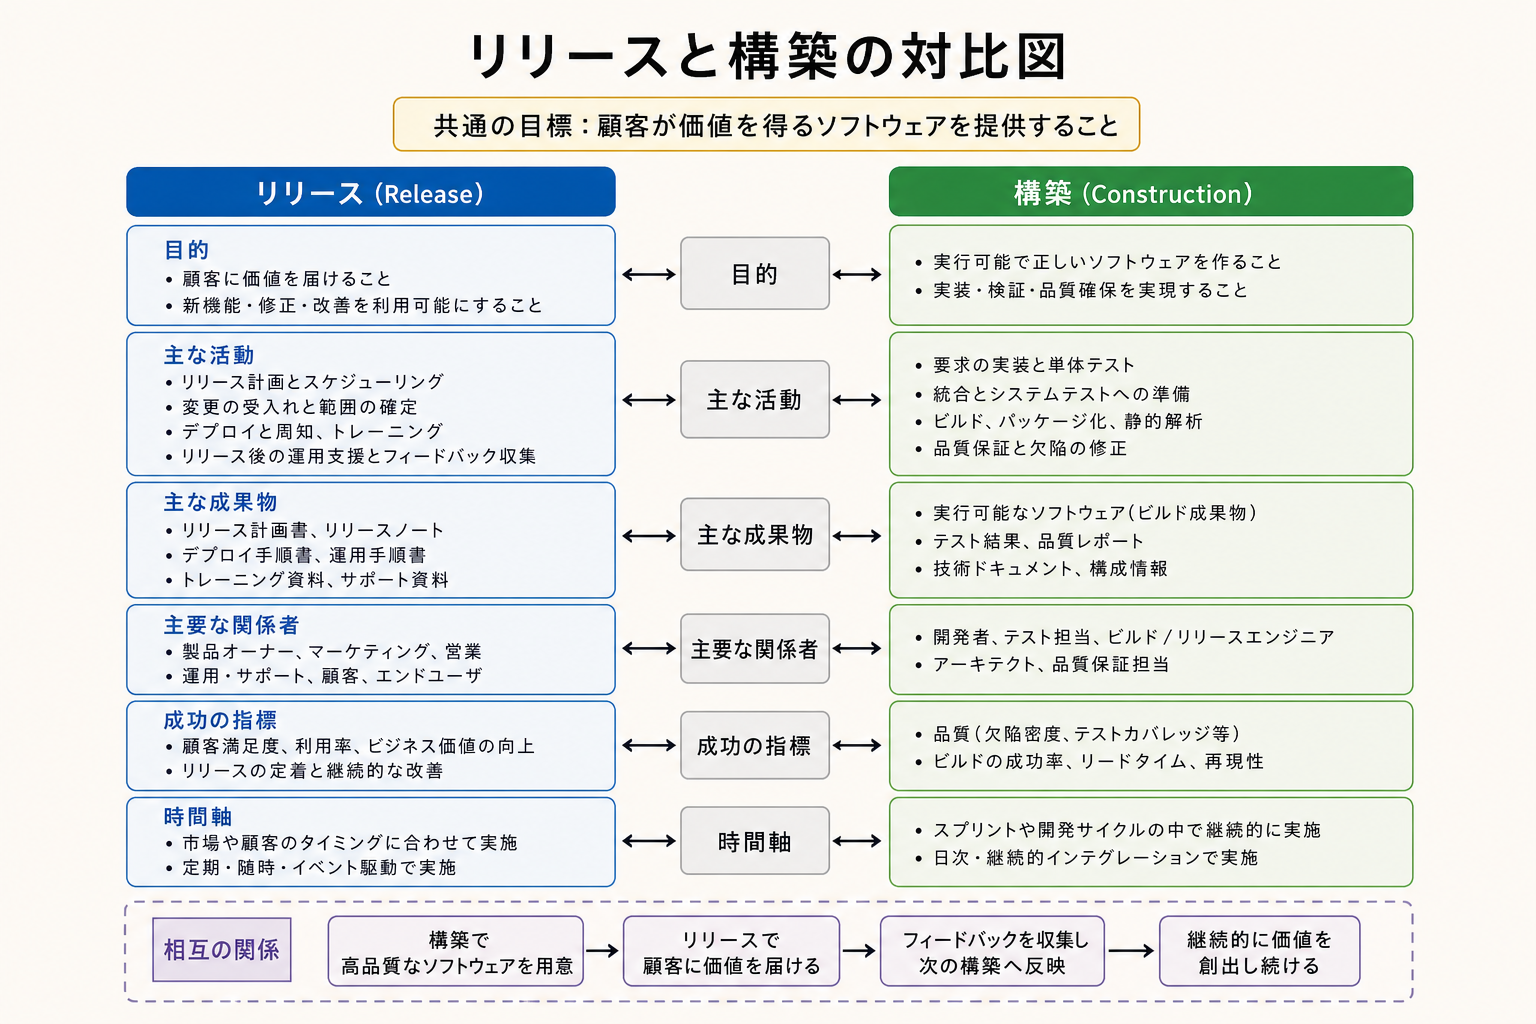
\includegraphics[width=0.96\linewidth]{assets/generated_figures/ch04/fig-ch04-07.png}}{\fbox{\parbox[c][48mm][c]{0.9\linewidth}{\centering 画像生成待ち\\段階的統合と継続的統合の流れ}}}
\par\smallskip
\refstepcounter{figure}\label{fig:ch04-07}図 \thefigure: 段階的統合と継続的統合の流れ
\end{center}
図 \thefigure は、段階的統合と継続的統合の流れを視覚的に整理したものである。
\par\smallskip

\subsubsection{クロスプラットフォーム開発と移行}

モバイルアプリケーションなどは、特定のプラットフォームに強く依存することが多い。たとえば、iOS と Android では、開発環境、API、利用できる機能、利用者体験が異なる。各プラットフォーム向けに別々に開発すると、費用と時間が増え、実装差も生まれやすい。

クロスプラットフォーム開発は、共通の言語やフレームワークで作り、複数のプラットフォームに出力する方法である。方式としては、共通言語から各プラットフォーム向けのネイティブアプリを生成する方法と、Web 技術で作った部分をネイティブのコンテナで包むハイブリッド方式がある。

既存アプリケーションを別のプラットフォームへ移す場合は、移行が必要になる。移行では、プログラミング言語の違い、API の違い、データ形式、テスト環境、利用者体験の差を考慮する必要がある。
